% 15 de mayo de 2018
\chapter{Presentación y discusión de la información}\label{ch:informacion}

El proceso de entrevistas fue realizado entre los meses de abril y septiembre
del año 2017.
Estas entrevistas fueron transcritas para su análisis en el texto.
Los elementos expresados por los participantes en las entrevistas fueron
codificados y organizados en las categorías y subcategorías que se pueden
observar en la figura~\ref{fig:categorias}.
Las entrevistas fueron codificadas empleando el programa ATLAS.TI en su versión
7.5.7 proceso que facilitó la categorización de la información recolectada a lo
largo de las entrevistas.

\begin{figure}
    \centering
    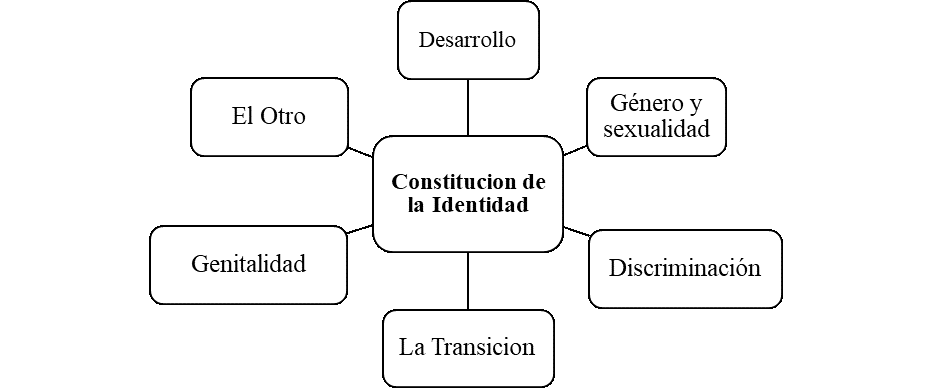
\includegraphics[width=0.75\textwidth]{categorias}
    \caption{Diagrama de categorías}\label{fig:categorias}
\end{figure}

A continuación realizaremos una descripción de cada una de ellas junto con los
verbatim que les dan origen.
Adicionalmente presentamos el razonamiento e interpretación que damos a cada
categoría y sus implicaciones caso a caso para el cumplimiento de los objetivos
de investigación.
El orden de presentación de las mismas fue elegido
según la frecuencia de manifestación en las entrevistas realizadas.

En la sección~\ref{sec:discusion}, realizamos una discusión y análisis punto a
punto de cada una de las categorías.

\section{Presentación de la información}

Como se puede ver resumido en la figura~\ref{fig:categorias}, hemos elaborado
seis (6) categorías. Dentro de estas categorías ‘La transición’ es uno de los
componentes identificados como constitutivo del proceso de construcción de la
identidad de las personas trans. Procederemos a explorar el contenido de cada
una de las categorías identificadas.

\subsection{Desarrollo}
Esta categoría se encuentra compuesta por elementos que abarcan desde etapas
tempranas de la niñez y del desarrollo.
Elementos como la relación del individuo con su escolaridad y compañeros de
clases.
También elementos de la constitución de los géneros que se hacen presentes
dentro de la pubertad y los conflictos que estos puedan causar a los
participantes
También incluye el papel que juega la familia dentro de la constitución de la
identidad así como la forma de aproximarse a los problemas.
Todos estos son elementos que pueden marcar la construcción de identidad de una
persona.

\begin{figure}
    \centering
    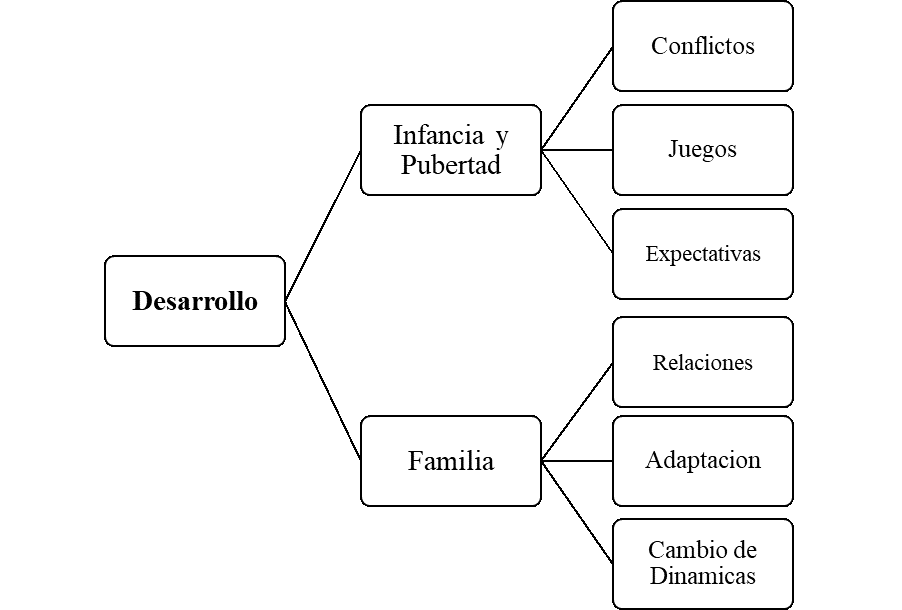
\includegraphics[width=0.75\textwidth]{desarrollo}
    \caption{Diagrama desarrollo y familia}\label{fig:desarrollo}
\end{figure}

En esta categoría confluyen elementos de conflicto así como las experiencias que
permitieron el manejo de los mismos en los participantes y que
consecuentemente se transformaron en estrategias de afrontamiento. Se debe tomar
en cuenta que en esta categoría se presentan los distintos tipos de relación
establecidas tanto en niveles académicos como familiares entre la infancia y
pubertad de los participantes.

Existen dos subcategorías dentro de este factor. Una de ‘infancia y pubertad’,
que reporta sobre las experiencias de desarrollo y formativas en la juventud, y
otra de ‘familia’. Esta habla acerca de la influencia de los lazos y ambiente
familiar durante el desarrollo.

\subsubsection{Infancia y pubertad}
Dentro de esta subcategoría se pueden
encontrar elementos que parecen ser transversales a lo largo de la vida del
individuo. Al ser tanto la infancia como la pubertad etapas tempranas de
desarrollo y constitución se pudo identificar elementos que parecen sentar las
bases para la forma otros elementos que le permiten al individuo constituirse
como persona. Entre estos elementos cabe resaltar la presencia de conflictos
como lo expresa el Sujeto 1 (verbatim):

\begin{verbatim}
…bueno me identificaba como niño pero me gustaba todo las cosas
de niña. De hecho siempre pedía al niño Jesús cosas de hembra, por ejemplo,
barbie, oso etcétera,  por su puesto jamás me traía lo que pedía y era muy
triste para mí, una era inocente y el niño Jesús me dejaba una carta explicando
que eso eran cosas de niña y me traía patineta bicicleta carrito y a mí no me
gustaba…
\end{verbatim}

Este elemento puede estar ligado al rechazo que pueden vivir, según lo expresado
por Sujeto 1 (verbatim):

\begin{verbatim}
…en la escuela era algo terrible por el bullying, pero yo
siempre imponía carácter y jamás me deje amedrentar por nada ni nadie.  De hecho
me agarre a golpes y me expulsaron por 10 días…
\end{verbatim}

O a tener su raíz en conflictos por la constitución de su identidad como lo
expresan con los siguientes verbatims.

Sujeto 1:
\begin{verbatim}
…yo lloraba porque no me entendía y me sentía mal.
\end{verbatim}

Sujeto 3:

\begin{verbatim}
…siempre era el raro del grupo…
\end{verbatim}

Y sujeto 2:

\begin{verbatim}
…me criticaban mucho como me vestía, pero es lo que me gusta.
\end{verbatim}

La aparición de estos conflictos entra en contacto con las aproximaciones a los
roles de género que suceden por primera vez en la infancia por medio de los
juegos y que perduran a lo largo de la vida de un individuo, como se evidencia
en el relato de Sujeto 1:

\begin{verbatim}
…a mí me decían que tenía que jugar con carritos y no con
muñecas porque eso es de niñas y yo no era una…
\end{verbatim}

\subsubsection{Familia}

\subsection{Género y sexualidad}

\subsubsection{Identidad de género}

\subsubsection{Hegemonía de género}

\subsubsection{Orientación sexual}

\subsection{Discriminación}

\subsubsection{Rechazo}

\subsubsection{Acoso / Bullying}

\subsubsection{Consecuencias}

\subsection{La transición}

\subsubsection{Transitar}

\subsubsection{Apariencia física}

\subsubsection{Conocimiento}

\subsection{Genitalidad}

\subsubsection{Lo esencial}

\subsubsection{Lo que se tiene}

\subsection{El Otro}

\subsubsection{Cómo me ven}

\subsubsection{Aspecto legal}

\section{Discusión}\label{sec:discusion}

\subsection{Desarrollo}

\subsubsection{Infancia y pubertad}

\subsubsection{Familia}
